\section{Object Stacking}
\label{app:stacking}

\subsection{Environment and expert}
The extension stacks a dynamic red 5~cm cube on a dynamic blue 5~cm cube with
the same Panda robot. Its 29D observation contains end-effector state, object
poses and velocities, gripper opening, and placement tolerance; actions remain
three Cartesian deltas plus a gripper command. Success requires physical
source--support contact, alignment and vertical separation within tolerance,
upright low-velocity cubes, an open gripper, robot retreat, and 20 consecutive
stable control steps. A deterministic finite-state expert approaches, grasps,
lifts, transports, aligns, lowers, releases, and retreats using real contacts.
It succeeds on 20/20 fixed and 100/100 randomized verification tasks.

Figure~\ref{fig:stacking-simulation-sequence} visualizes these physical stages
within one successful rollout. In the last frame the gripper has retreated and
the environment's persistent success detector is true after 21 stable control
steps.

\begin{center}
\begin{minipage}{\linewidth}
  \centering
  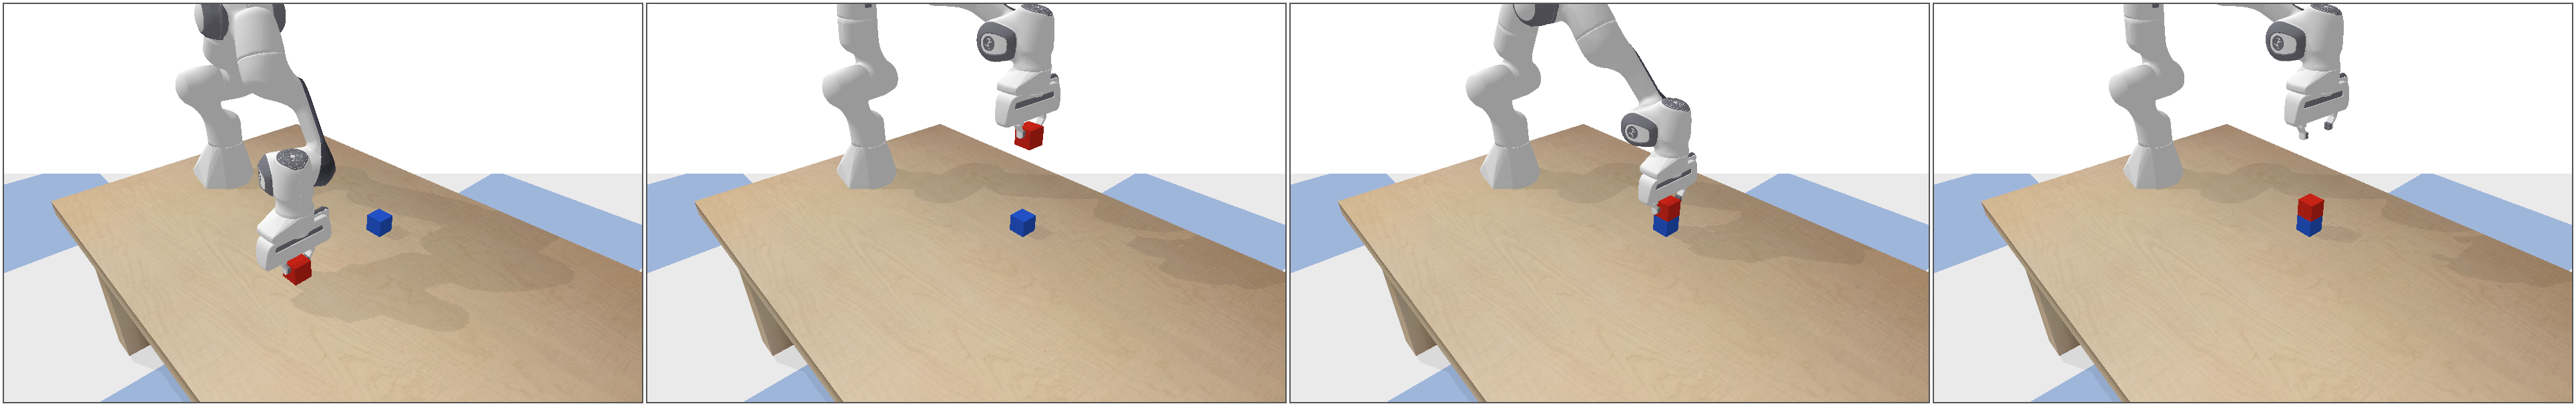
\includegraphics[width=\textwidth]{figures/stacking_simulation_sequence.png}
  \makeatletter
  \def\@captype{figure}
  \makeatother
  \caption{Real PyBullet states from one successful deterministic stacking
  expert rollout: (a) finger grasp of the red source cube, (b) lifted source
  aligned above the dynamic blue support cube, (c) physical source--support
  contact during release, and (d) the stable stack after robot retreat. The
  final frame satisfies \texttt{env.is\_success()} with source--support contact
  and 21 consecutive stable control steps.}
  \label{fig:stacking-simulation-sequence}
\end{minipage}
\end{center}

\subsection{Dataset and behavior cloning}
The frozen dataset contains 300 successful demonstrations and 70,678
transitions, split into 240 training and 60 validation trajectories. Initial
source and support positions vary within conservative reachable ranges, and
placement tolerance is uniform in $[0.012,0.015]$~m. The original scaled BC
obtains 1/100 development successes. Diagnostic analysis identifies large
ALIGN error, phase imbalance, premature release, and closed-loop state shift.
The selected S4.5 representation retains 29 dimensions but replaces source
position with source-minus-end-effector and support position with
source-minus-support. ALIGN, LOWER\_TO\_PRECONTACT, LOWER\_TO\_CONTACT, and
RELEASE transitions receive fivefold effective emphasis. This development
policy obtains 9/100; it is distinct from the matched S6 Uniform models.

\subsection{Difficulty analysis}
Stacking task difficulty replaces object--goal distance with source--support
distance and uses inverse placement tolerance. The Spearman correlations in
Figure~\ref{fig:stack-corr} are $0.802$ (Task--Expert), $-0.102$
(Task--Learner), and $-0.058$ (Expert--Learner). Task and expert scores remain
related, but learner disagreement is weaker than in pick-and-place.

\begin{figure}[!htbp]
  \centering
  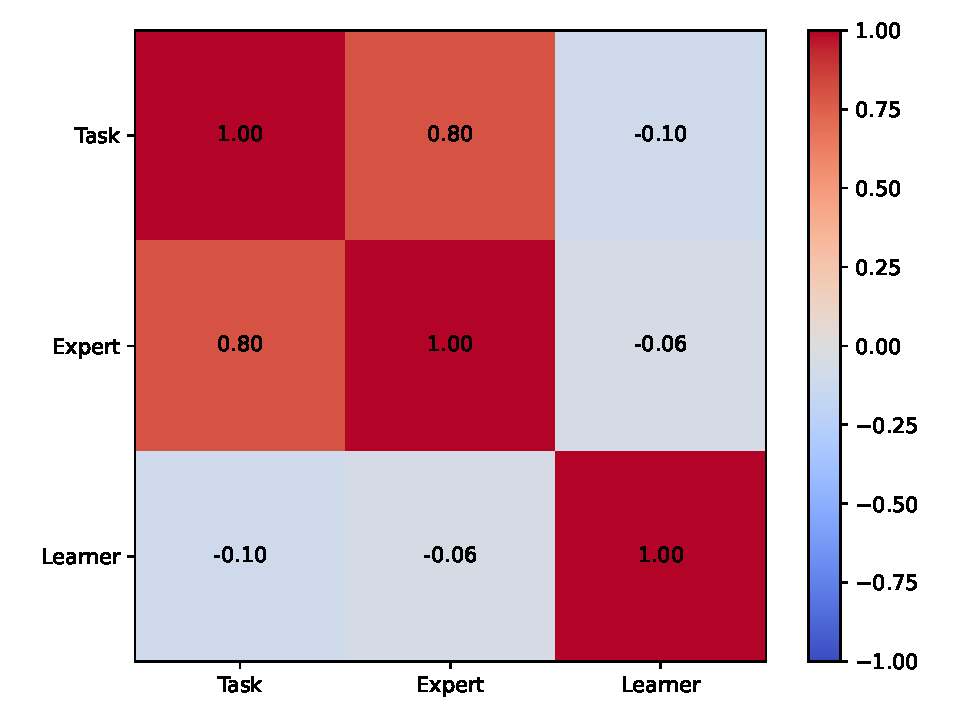
\includegraphics[width=.55\linewidth]{figures/stacking_difficulty_correlation.pdf}
  \caption{Stacking difficulty-score Spearman correlations.}
  \label{fig:stack-corr}
\end{figure}

\subsection{Curriculum results}
All methods use the relative representation and phase emphasis, with emphasis
restricted to the eligible trajectories at each stage. Table~\ref{tab:stack}
reports 200 frozen Fresh-ID tasks (seed 65478). Uniform is strongest, although
all methods are near the performance floor and seed variability remains
material. This exploratory comparison cannot establish a robust reversal of
the pick-and-place ordering.

\begin{table}[!htbp]
\centering
\caption{Stacking final results and development AUC, mean $\pm$ sample SD over
three seeds. Bold marks only the largest observed mean.}
\label{tab:stack}
\small
\begin{tabular}{lcc}
\toprule
Method & Fresh-ID success (\%) & Development AUC \\
\midrule
Uniform & $\mathbf{8.33\!\pm\!5.75}$ & $0.03792$ \\
Task & $3.50\!\pm\!1.32$ & $0.01808$ \\
Expert & $2.50\!\pm\!2.18$ & $0.02667$ \\
Learner & $1.50\!\pm\!1.50$ & $0.01408$ \\
Reverse Learner & $2.50\!\pm\!2.00$ & $0.01175$ \\
\bottomrule
\end{tabular}
\end{table}

\begin{figure}[!htbp]
  \centering
  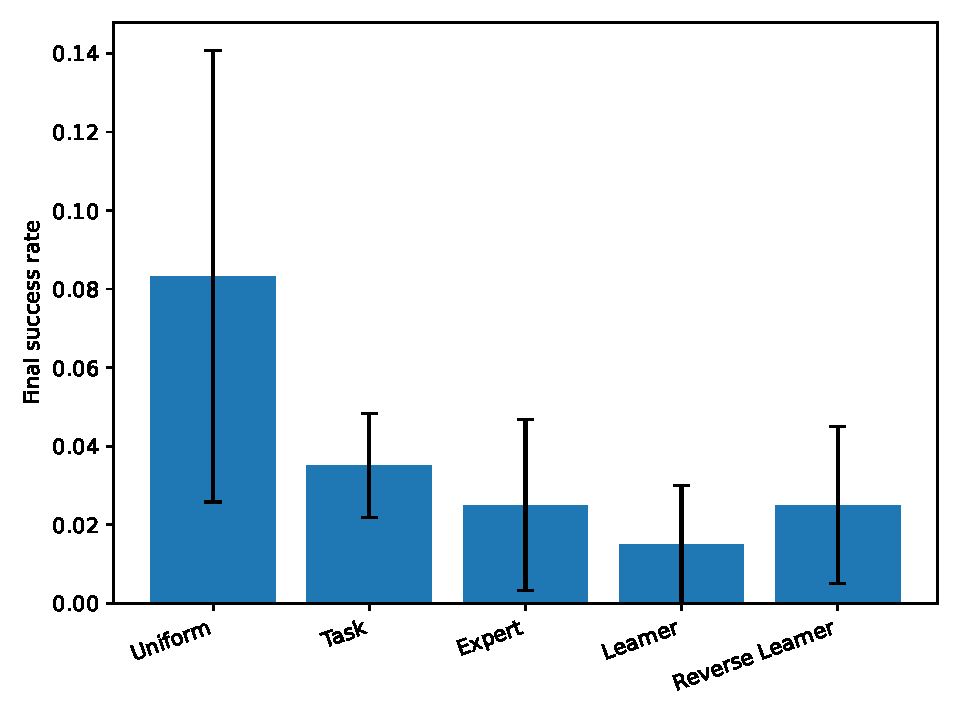
\includegraphics[width=.55\linewidth]{figures/stacking_final_success.pdf}
  \caption{Stacking Fresh-ID success at the predefined 20,600-update
  checkpoint. Error bars show sample standard deviation across three seeds.}
  \label{fig:stack-final}
\end{figure}

\clearpage
\begin{center}
\begin{minipage}{\linewidth}
  \centering
  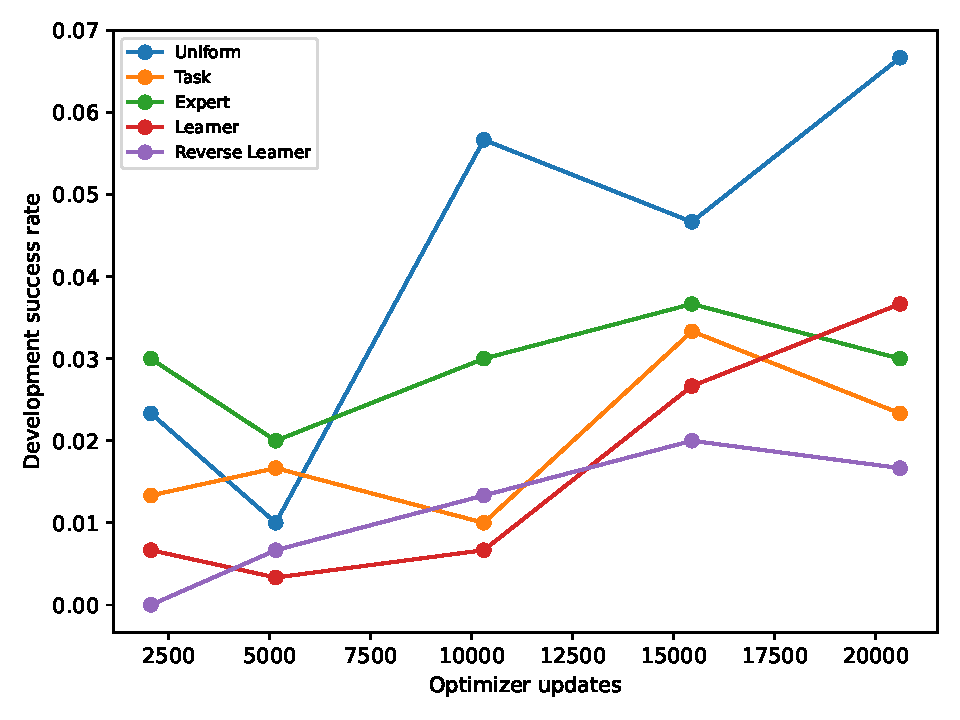
\includegraphics[width=.64\linewidth]{figures/stacking_learning_curves.pdf}
  \makeatletter
  \def\@captype{figure}
  \makeatother
  \caption{Mean stacking development learning curves across three seeds on
  100 frozen tasks; no uncertainty bands are shown.}
  \label{fig:stack-curves}
\end{minipage}
\end{center}

\subsection{Failure analysis}
Failure categories are derived from physical events observed over the rollout.
A grasp/lift failure never raises the source sufficiently; transport/alignment
failure does not move it toward the support; placement/contact failure never
establishes source--support contact; and post-release instability reaches
contact but fails persistent success after opening and retreat. Across all
three seeds, placement/contact dominates (297 failures for Uniform), followed
by post-release instability (195). Reverse Learner has 279 placement/contact
and 245 instability failures. These categories are diagnostic event summaries,
not mutually causal explanations.

\subsection{Cross-task limitations}
Pick-and-place and stacking use 10D and 29D observations respectively.
Stacking additionally uses relative coordinates and phase-balanced training,
and demands persistent contact after release. Overall success is near floor,
so the absence of a curriculum gain is not a strong negative replication.
Only three seeds are available, and the curves do not establish complete
convergence. The cross-task contrast is exploratory and cannot establish that
task identity alone changes the preferred schedule.

\newpage
